\section{Oggetti in gioco}
In questa sezione vengono descritti i diversi aspetti tecnologici, che vanno dalla raccolta delle informazioni fino al aspetto tecnologico con cui viene trattato il dato.

\subsection{Architettura delle Smart City}
Una Smart City è costituita dai seguenti livelli gerarchici:\cite{smart:city_cybersecurity_privacy_cap4}
\begin{itemize}
  \item \textbf{Livello 1 - Ambiente} include tutte le caratterisciche ambientali della cittò;
  \item \textbf{Livello 2 - Infrastruttura Hardware (no ICT based)} è costituita da tutte le infrastrutture urbane quali edifici, ponti, strade, viadotti, acqueddotti ecc.;
  \item \textbf{Livello 3 - Infrastruttura Hardware (ICT based)} riguarda tutto l'hardware con cui vengono raccolte e prodotte tutte le informazioni come l'infrastruttura IoT, sensori, attuatori, reti di comunicazione, ecc.;
  \item \textbf{Livello 4 - Smart Service} sono tutti quei servizi direttamente prodotti dall'infrastruttura hardware e software come smart safety, intelligent transportation, smart government, smart water, ecc.;
  \item \textbf{Livello 5 - infrastruttura Software} costituisce l'insieme di persone fisiche o utenti finale della città che usufruiscono dei servizi smart.
  
\end{itemize}


\subsection{Internet of Things}
La raccolta di informazioni all'interno di una Smart City avviene attraverso una serie di oggetti chiamati sensori\footnote{I sensori sono dispositivo meccanico, elettronico o chimico, che in apparecchiature o meccanismi rileva i valori di una grandezza fisica e ne trasmette le variazioni a un sistema di misurazione o di controllo.}, sparsi in giro per la città. Questi sonseori sono connessi a internet attraverso specifici protocolli di comunicazione. Questo approccio alla raccolta di dati viene chiamato IoT acronimo di Internet of Things (internet delle cose).
All'interno di una Smart City si possono trovare sensori per il rilevamento della qualità dell'aria come il pm10 e pm2.5\footnote{PM sta a indicare il particulate matter e sta ad indicare l'insieme delle sostanze sospese in aria, precisamente il particolato è l'inquinante oggi più frequente nelle aree urbane, ed è composto di particelle solide o liquide disperse nell'atmosfera.}, il gps\footnote{Il gps, acronimo di global positioning system, sistema di posizionamento globale, è un sistema di posizionamento e navigazione satellitare militare statunitense che una rete dedicata di satelliti artificiali in orbita attorno alla terra.}, questo sensore vienen sopratutto utilizzato per monitorare gli spostamenti dei vai mezzi pubblici oppure bike e car sharing.

\subsection{Criteri architetturali di una smart city}
riferimento\cite{smart_city_architetture}
FIWARE come framework aperto 

\subsection{Partecipazione e collaborazione}
Per partecipazione e collaborazione si intende l’iniziativa spontanea del cittadino nel mantenimento dello stato ottimale dei servizi o del arredo urbano attraverso appositi strumenti forniti dall'amministrazione locale. Questo può avvenire fornendo al cittadino strumenti di ticketing per segnalare eventuali guasti o danni ad impianti pubblici come installazione di pubblica illuminazione o strade rotte. In questo modo il comune o chi di dovere abbia conoscenza della manutenzione richiesat all'interno della città.

In italia, la società Citelum SA, società francese del gruppo EDF che si occupa di efficentamento energetico e pubblica illuminazione, ha distribuito ad oltre duecento comune del centro nord Itala, un sistema di ticketing, rivolto ai cittadini, per la segnalazione di guasti o anomalie agli impianti di pubblica illuminazione e alla segnaletica semaforica, tramite l'utilizzo del proprio smartphone. Ogni istallazione luminosa o punto luce (palo della luce o semaforo), è dotata di una etichetta identificativa con relativo qr-code\footnote{Il qr-code è un codice a barre bidimensionale (o codice 2D), composto da moduli neri disposti all'interno di uno schema bianco di forma quadrata, impiegato tipicamente per memorizzare informazioni generalmente destinate a essere lette tramite uno smartphone.}, l'utente, dopo aver scansionato il qrcode, viene reindirizzato alla pagina della segnalazione, in figura 1.10 un esempio di segnalazione preso da un fermo immagine del video di presentazione della Smart City di Lonato promossa sempre da Citelum SA\cite{citelum_smart_city_lonato}.
\begin{figure}[h!]
    \centering
        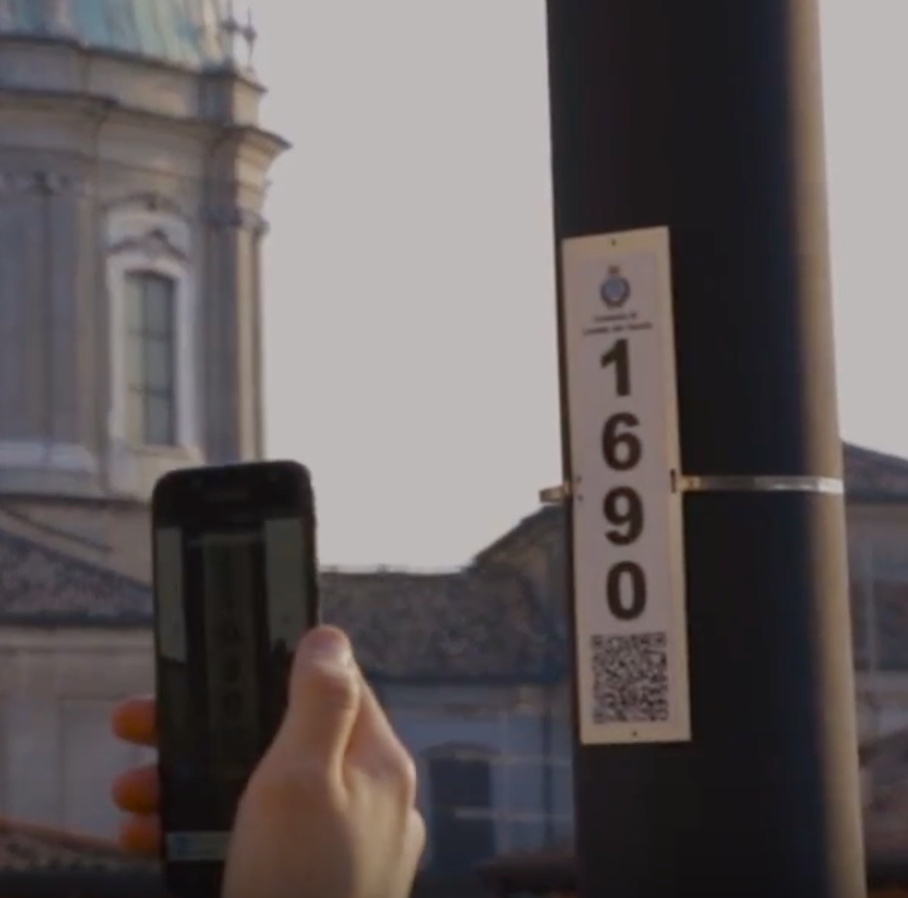
\includegraphics[width=150bp]{img/faro/faro_qrcode.png}
            \quad
        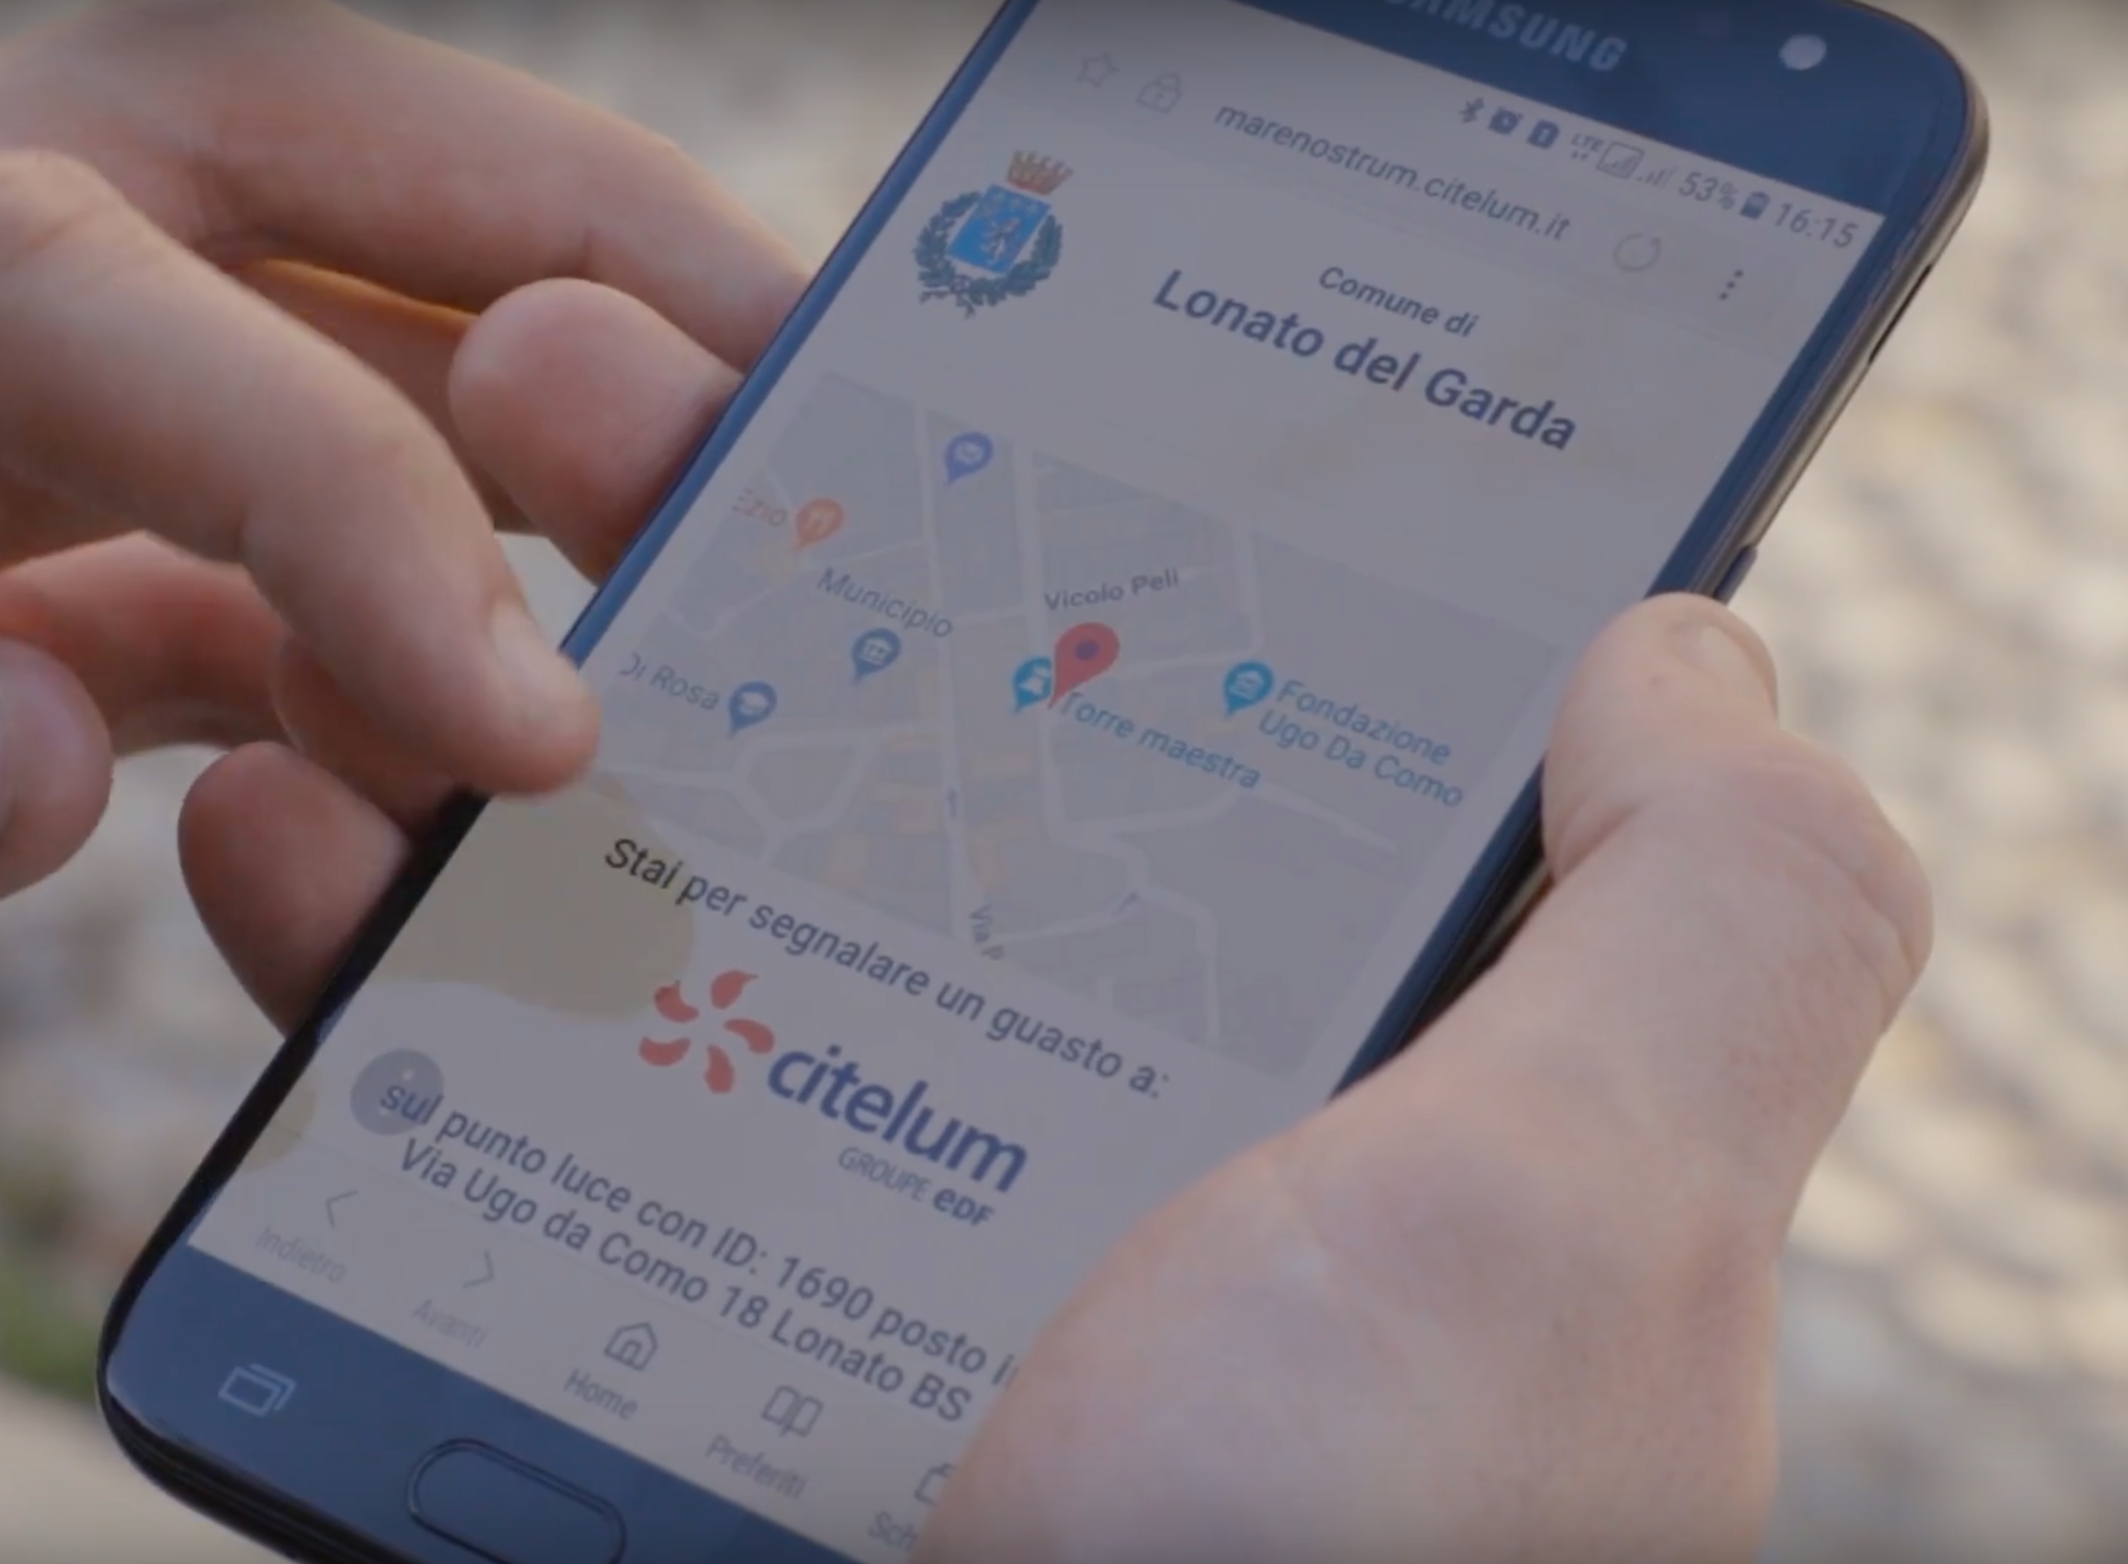
\includegraphics[width=150bp]{img/faro/faro_openpage.png}
            \quad
        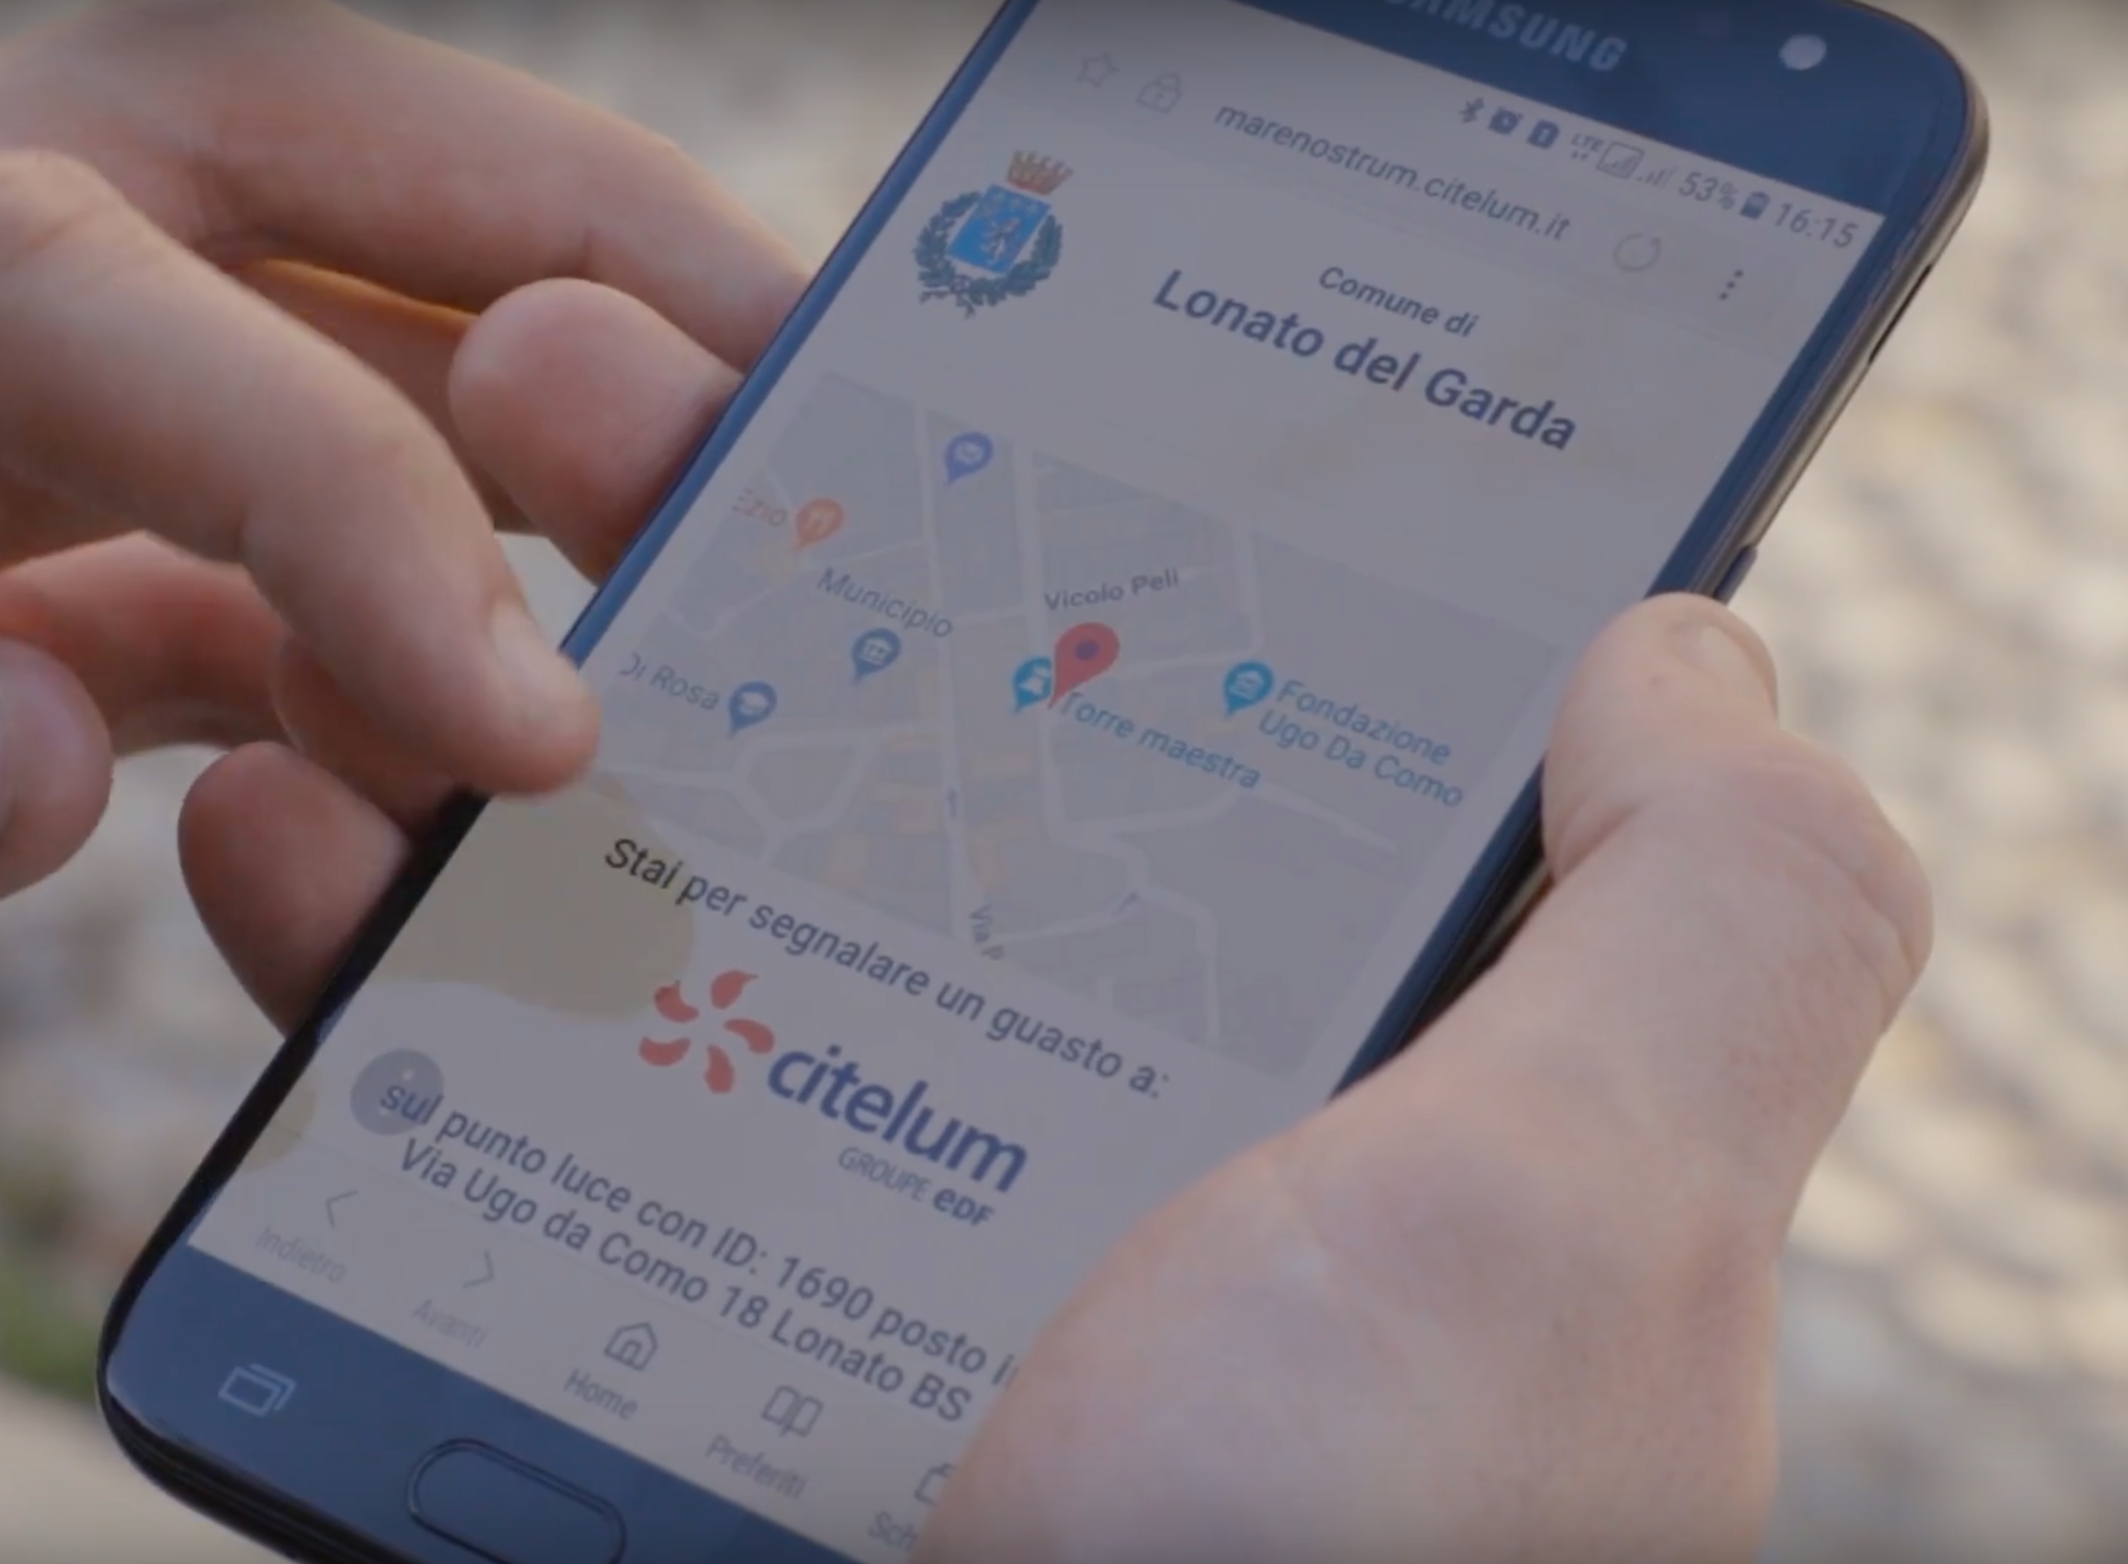
\includegraphics[width=150bp]{img/faro/faro_segnalazione_1.png}
            \quad
        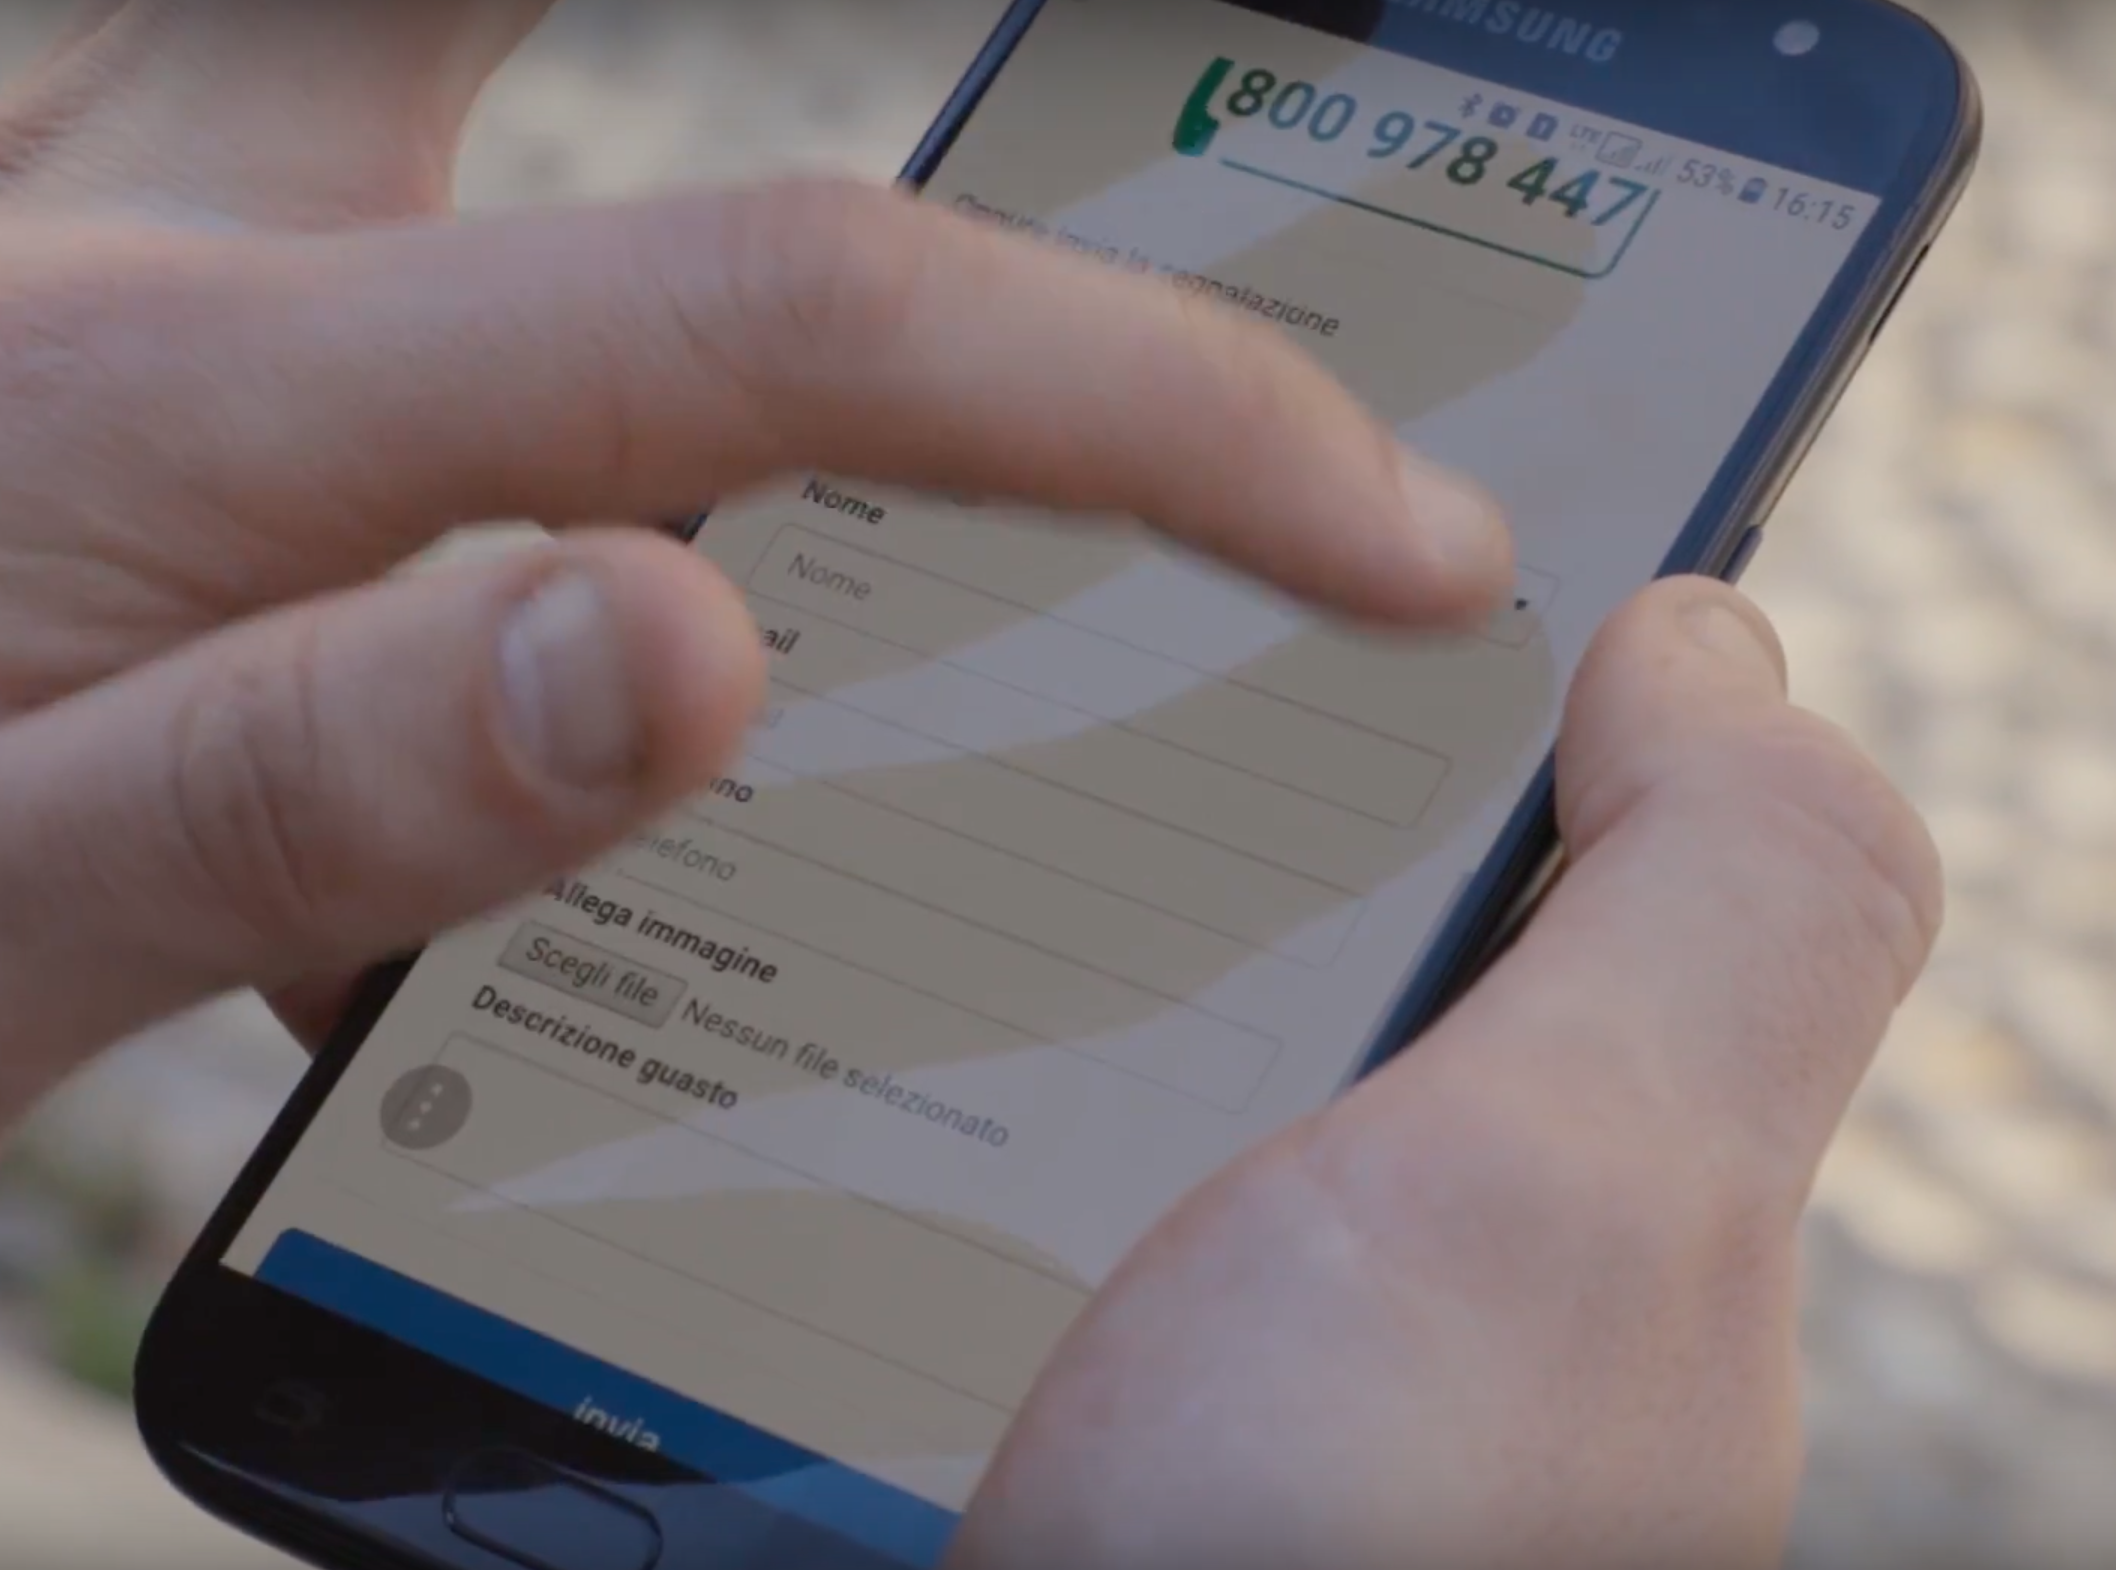
\includegraphics[width=150bp]{img/faro/faro_segnalazione_2.png}
    \caption{Esempio di apertura di un ticketing}
\end{figure}
Una volta scansionato il qr-code, con un apposita applicazione per la lettura dei qr-code, il sistema chiederà all'utente di essere reindirizzato ad una pagina web, tale pagina è composta da una mappa georeferenziata con il punto luce, i dati relativi alla composizione dell'impianto semaforico e un form di registrazione dove vene richiesto di inserire:
\begin{wrapfigure}{r}{0.3\textwidth}
    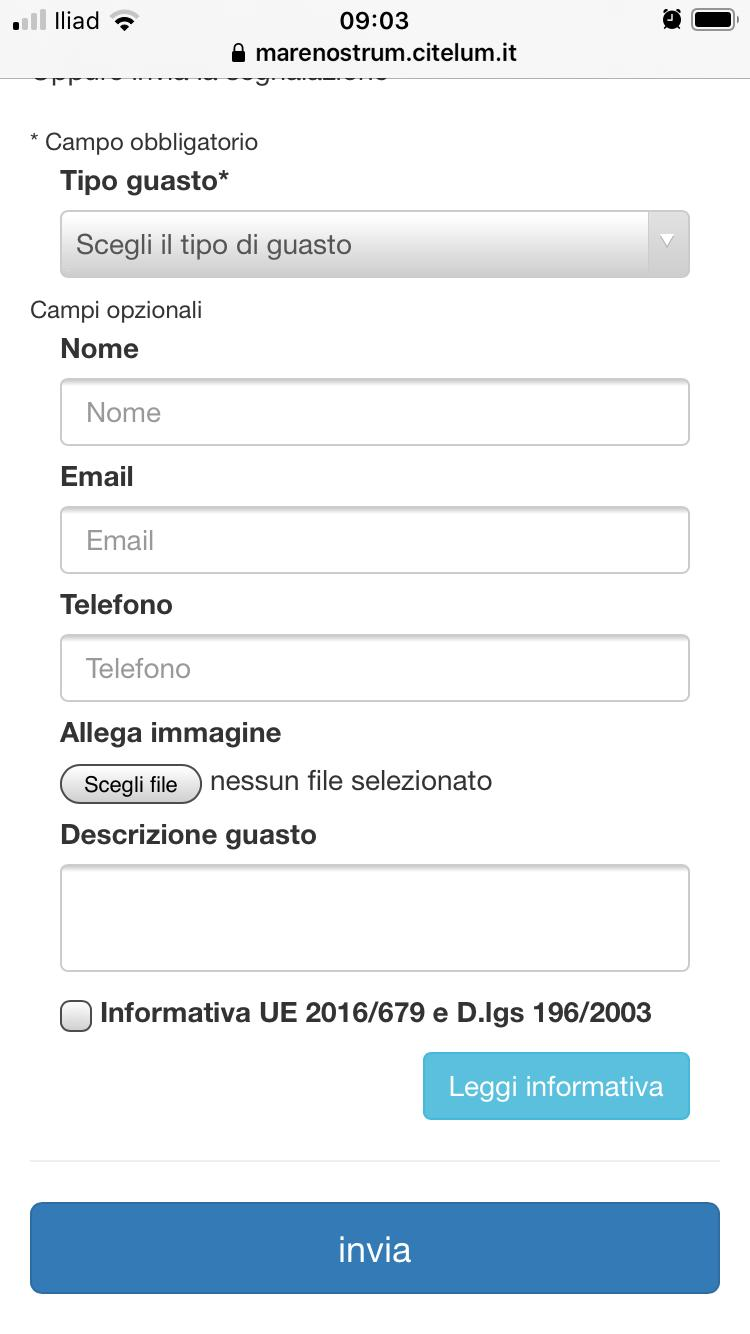
\includegraphics[width=0.40\textwidth]{img/faro/qrlonato2.jpg}
\end{wrapfigure}
\begin{itemize}
  \item \textbf{Nome del segnalante}
  \item \textbf{Email del segnalante}
  \item \textbf{Tipo guasto scelto da una lista}
  \item \textbf{Allegare una foto dell'impianto} (Opzionale)
  \item \textbf{Spunta sull'informativa UE2016/679 e D.lgs 196/2003}
\end{itemize}

L'esempio di for viene mostrato nell'immagine affianco. Dopo aver compilato il form, al click su "Invia", l'utente invierà una segnalazione alla società incaricata alla manutenzione della pubblica illuminazione relativo a quel comune.

